\section{Versuchsaufbau/-durchführung}

\subsection{Versuchsaufbau}

Der Versuchsaufbau ist in Abbildung \ref{fig: versuchsaufabu} dargestellt.
Zusehen ist dort das Zählrohr und die nachgeschaltete Elektronik.
Die Elektronik umfasst einen Verstärker, ein Oszilloskop und
ein Zählwerk. Das Zählwerkt gibt die Anzahl der eintreffenden Teilchen
an. Der vor dem Zählrohr geschaltete Kondensator $C$ koppelt den eintreffenden
Stromimpuls vom Zählrohr ab.
\begin{figure}
  \centering
  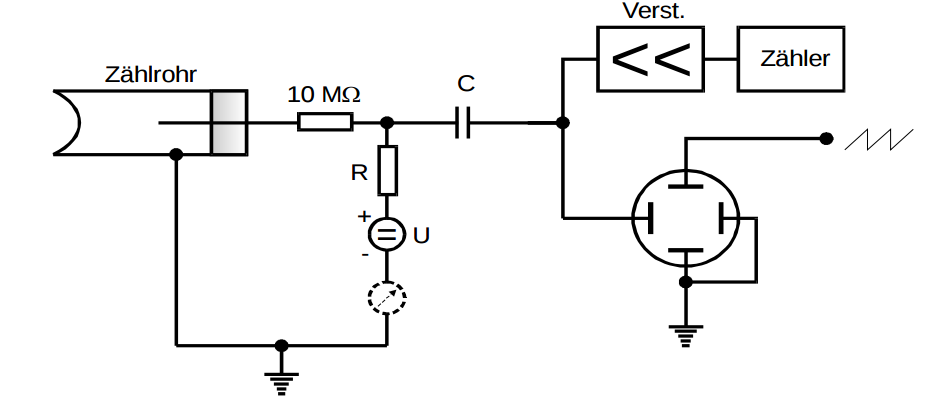
\includegraphics[width=0.6\textwidth]{bilder/aufbau.png}
  \caption{Schematische Darstellung des Aufbaus für die Untersuchung eines Geiger-Müller-Zählrohrs \cite{anleitung703}.}
  \label{fig: versuchsaufabu}
  \end{figure}
\subsection{Versuchsdurchführung}

\subsubsection{Aufnahme der Charakteristika des Zählrohres}

Nachdem eine $\beta$-Quelle vor das Fenster des Zährohers plaziert wurde
kann die Zählrate in Abhängigkeit von der Betriebspannung $U$ gemessen.
Es werden nun Zählraten für den Bereich $U\in\left[300, 700\right] \, \si{\volt}$
untersucht. Die Zählrate wird in einem Zeitraum von $\SI{60}{\second}$ gemessen.


\subsubsection{Ostillographische Messung Tot- und Erholungszeit}
Man schließt zunächst das Geiger-Müller-Zählrohr an ein
Oszilloskop an. Das Oszilloskop zeigt nun den in Abbildung \ref{}
dargestellten Spannungsverlauf an. Mit einer geeigneten Zeitskalierung am Oszilloskop
liest man nun die Tot- und Erholungszeit ab.
Die Prozedur wird für fünf verschiedene Spannungen durchgeführt.

\subsection{Bestimmung der Totzeit mit der Zwei-Quellen-Methode}
Auf Grund der Totzeit $T$ eines Geiger-Müller-Zähler, gibt es immer einen
Unterschied zwischen der wahren und der gemessenen Zählrate.
Der Zusammenhang zwischen der gemessenen Zählrate $N\ua{r}$ und
wahren $N\ua{w}$ lautet:
\begin{equation}
  \label{eq:wahre_zaehlrate}
  N\ua{w}=\frac{N\ua{r}}{1-TN\ua{r}}.
\end{equation}
Betrachtet man nun zwei unterschiedliche Präparate ist eine
Bestimmung der Totzeit möglich.Dazu werden, bei $\SI{480}{\volt}$ und in eiem Zeitraum $\SI{60}{\second}$ eine neue
$\ce{^{204}Tl}$ und einer alte $\ce{^{204}Tl}$ Probe untersucht.
Zunächst wird die Zählrate der einzelnen bestimmt $N_1$ und $N_2$, danach die
Summe aus beiden $N_1+N_2$. Beim einsetzen der zweiten Probe, darf die Position der
ersten Probe nicht verändert werden.
Auf Grund der Totzeit gilt der Zusammenhang
\begin{equation}
  \label{eq:totzeit_summe}
  N_{1+2}<N_1+N_2,
\end{equation}
mit diesem kann dann die Totzeit zu
\begin{equation}
  \label{eq:totzeit}
  T\approx \frac{N_1+N_2-N_{1+2}}{2N_1N_2}
\end{equation}
genährt werden.

\subsubsection{Messung der pro Teilchen vom Zählrohr feigesetzte Ladunfsmenge}
Die vom eindrigenden Teilcehn vom Zählrohr freigesetzte Ladungsmenge kann mit

\begin{equation}
  \label{eq:lafung_pro_teilchen}
  I=\frac{\Delta Q}{\Delta t} N
\end{equation}
berechnet werden ($N$ ist die Anzahl der Teilchen).
Durch Messung des Stroms mit Hilfe eines empfindlichen Messgerätes,
kann die Ladungsenge in Abhängigkeit von der Spannung $U$ untersucht werden.
Der Spannungbereich liegt bei $U\in\left[300, 700\right] \, \si{\volt}$.
